% !TeX program = xelatex
% ============================================================================
%  第 1 课　先导课：抽象代数是什么
% ----------------------------------------------------------------------------
%  编译        XeLaTeX，编译两遍（顶部导航栏的节名与小圆点需要第二遍才更新）
%  样式        ../../00-共享/preamble.tex（想改配色、字体只改那一个文件）
%  校徽        ../../00-共享/logo_white.png（preamble 里的 \graphicspath 已配好）
%  图片        暂时用 \imgph{说明} 占位；有图以后换成
%              \includegraphics[width=0.7\textwidth]{图片名}
% ============================================================================

\documentclass[10pt]{beamer}
% ============================================================================
%  讲义样式文件 —— 字体 / 配色 / 校徽栏 / 顶部导航栏 / 页脚 / 常用方框
%  所有个性化设置都集中在这里，改一次即可用于所有讲义
%
%  用法：主文件里写
%      \documentclass[10pt]{beamer}
%      \input{preamble.tex}
%  依赖：同目录下的 logo_white.png（顶部校徽）
%  编译：必须用 XeLaTeX，而且必须编译两遍
%        （顶部导航栏的节名与小圆点记录在 .nav 文件里，只编一遍不会更新）
% ============================================================================
\usepackage{ctex}  % 支持中文
\usepackage{amsmath, amssymb}  % 数学公式支持
\usepackage{fontspec}  % 字体设置
\usepackage{unicode-math}  % 支持Unicode数学字体
\usepackage{xcolor}  % 颜色
\usepackage{tikz}  % 用于绘制页脚色条
\usepackage{booktabs}  % 表格

% 图片搜索路径 ------------------------------------------------------------------
% 校本课的资料分目录存放，本文件可能被 02-课件/第XX课/ 、03-讲义/ 下的主文件调用，
% 这里把几种可能的相对位置都列上，logo_white.png 放在 00-共享/ 即可被找到。
% 最后一项 00-共享/图片/ 是给 \imgfig 用的插图目录（图与课件不在同一层，靠它找到）。
\graphicspath{{./}{./图片/}{../../00-共享/}{../00-共享/}{00-共享/}{../../00-共享/图片/}{../00-共享/图片/}{00-共享/图片/}}

% 设置字体
\setCJKmainfont{SimSun}  % 设置中文字体为宋体
\setmainfont{Palatino Linotype}  % 设置英文字体为Palatino Linotype
\setmathfont{Latin Modern Math}  % 设置数学字体为Latin Modern Math
% 注意：beamer 默认把正文字体族设成无衬线（sans），Windows 下对应的中文字体是
% 微软雅黑，所以上面这行 SimSun 目前对正文不起作用。想让正文变成宋体，取消
% 下面这行的注释即可（标题栏、页脚、方框标题不受影响）。
% \renewcommand{\familydefault}{\rmdefault}

% 定义颜色 - 均为绿色系
\definecolor{maingreen}{RGB}{34,139,34}  % 森林绿（导航栏底色）
\definecolor{lightgreen}{RGB}{240,255,240}  % 蜜瓜白（帧标题栏底色）
\definecolor{accentgreen}{RGB}{46,139,87}  % 海绿（强调色）
\definecolor{textgreen}{RGB}{0,128,0}  % 纯绿（标题文字）
\definecolor{darkgreen}{RGB}{20,90,20}  % 深绿（顶部校徽栏底色）

% 设置Beamer主题
\usetheme{default}
\usecolortheme{default}

% 自定义主题
\setbeamercolor{background canvas}{bg=white}
\setbeamercolor{frametitle}{fg=textgreen, bg=lightgreen}
\setbeamercolor{title}{fg=textgreen}
\setbeamercolor{subtitle}{fg=textgreen}
\setbeamercolor{section in toc}{fg=accentgreen}
\setbeamercolor{normal text}{fg=black}
\setbeamercolor{structure}{fg=accentgreen}
\setbeamercolor{itemize item}{fg=accentgreen}
\setbeamercolor{itemize subitem}{fg=accentgreen}
\setbeamercolor{itemize subsubitem}{fg=accentgreen}
\setbeamercolor{block title}{fg=white, bg=accentgreen}
\setbeamercolor{block body}{bg=lightgreen}
% example 环境（底层是 exampleblock）用的是独立的一组颜色名，default 配色主题下
% 它们的底色是空的，所以只设 block 的话“例”会变成一行没有框的标题，这里接过来
\setbeamercolor{block title example}{parent=block title}
\setbeamercolor{block body example}{parent=block body}

% ==================== 常用定理类方框（五类配色）====================
% 五类各自的标题条底色，正文底色由同色自动调浅（!8!white）
\definecolor{boxThm}{RGB}{20,90,20}    % 一、定理类：深绿
\definecolor{boxDef}{RGB}{46,139,87}   % 二、定义类：海绿
\definecolor{boxExm}{RGB}{34,139,34}   % 三、例题类：森林绿
\definecolor{boxPrf}{RGB}{85,107,47}   % 四、过程类：橄榄绿
\definecolor{boxNote}{RGB}{0,121,107}  % 五、注记类：青绿

% 方框本体：先套本类配色，再调用 beamer 的 block（改动只在环境内部生效）
\newcommand{\gbox}[2]{%
  \setbeamercolor{block title}{fg=white,bg=#1}%
  \setbeamercolor{block body}{bg=#1!8!white}%
  \begin{block}{#2}}
\newcommand{\gboxend}{\end{block}}
% 标题后的可选补充名：\begin{theorem}[勾股定理] → 定理（勾股定理）
\newcommand{\gsub}[1]{\ifx\relax#1\relax\else（#1）\fi}


% 一、定理类（定理/推论/性质/命题/引理）
\renewenvironment{theorem}[1][]{\gbox{boxThm}{定理\gsub{#1}}}{\gboxend}
\renewenvironment{corollary}[1][]{\gbox{boxThm}{推论\gsub{#1}}}{\gboxend}
\newenvironment{character}[1][]{\gbox{boxThm}{性质\gsub{#1}}}{\gboxend}
\newenvironment{proposition}[1][]{\gbox{boxThm}{命题\gsub{#1}}}{\gboxend}
\renewenvironment{lemma}[1][]{\gbox{boxThm}{引理\gsub{#1}}}{\gboxend}

% 二、定义类（定义/公理）
\renewenvironment{definition}[1][]{\gbox{boxDef}{定义\gsub{#1}}}{\gboxend}
\newenvironment{axiom}[1][]{\gbox{boxDef}{公理\gsub{#1}}}{\gboxend}

% 三、例题类（例/练习/习题）
\renewenvironment{example}[1][]{\gbox{boxExm}{例\gsub{#1}}}{\gboxend}
\newenvironment{exercise}[1][]{\gbox{boxExm}{练习\gsub{#1}}}{\gboxend}
\newenvironment{homework}[1][]{\gbox{boxExm}{习题\gsub{#1}}}{\gboxend}

% 四、过程类（证明/解/法1~法4）
\renewenvironment{proof}[1][]{\gbox{boxPrf}{证明\gsub{#1}}}{\qedsymbol\gboxend}
\newenvironment{jie}[1][]{\gbox{boxPrf}{解\gsub{#1}}}{\gboxend}
\newenvironment{way1}[1][]{\gbox{boxPrf}{法1\gsub{#1}}}{\gboxend}
\newenvironment{way2}[1][]{\gbox{boxPrf}{法2\gsub{#1}}}{\gboxend}
\newenvironment{way3}[1][]{\gbox{boxPrf}{法3\gsub{#1}}}{\gboxend}
\newenvironment{way4}[1][]{\gbox{boxPrf}{法4\gsub{#1}}}{\gboxend}

% 五、注记类（经验总结/注/值得注意的是/分析/提示）
\newenvironment{experience}[1][]{\gbox{boxNote}{经验总结\gsub{#1}}}{\gboxend}
\newenvironment{zhu}[1][]{\gbox{boxNote}{注\gsub{#1}}}{\gboxend}
\newenvironment{att}[1][]{\gbox{boxNote}{值得注意的是\gsub{#1}}}{\gboxend}
\newenvironment{analyse}[1][]{\gbox{boxNote}{分析\gsub{#1}}}{\gboxend}
\newenvironment{hint}[1][]{\gbox{boxNote}{提示\gsub{#1}}}{\gboxend}

% 顶部导航栏（miniframes 主题：显示各节名称 + 帧圆点）
% 节名与圆点记录在 .nav 文件中，改动章节后需要编译两遍才会同步
\useoutertheme[subsection=false]{miniframes}
\setbeamercolor{section in head/foot}{fg=yellow, bg=maingreen}
\setbeamercolor{mini frame}{fg=yellow, bg=maingreen}
\setbeamercolor{mini frame in current subsection}{fg=yellow, bg=accentgreen}

% 顶部校徽栏：位于导航栏上方，宽度与帧标题栏一致（整页宽）
% 校训用的楷体：ctex 的 \kaishu 在本机指向未安装的 Adobe 楷体，这里直接指定系统楷体
\setCJKfamilyfont{kaiti}{KaiTi}
\setbeamercolor{logo bar}{fg=white, bg=darkgreen}
\addtobeamertemplate{headline}{%
  \begin{beamercolorbox}[wd=\paperwidth,ht=0.84cm,dp=0.20cm,leftskip=0.25cm,rightskip=0.25cm]{logo bar}%
    % -0.035cm：色条内容默认坐在基线上，会比栏的中线略高，下移这一点使其上下居中
    \raisebox{-0.035cm}{
\includegraphics[height=0.72cm]{logo_white.png}}%
    % 右侧校训：字体为上面定义的楷体，也可改为 \insertsectionhead（当前节名）、\inserttitle（章节名）等
    % 0.375cm = 校徽中线（0.36cm）加汉字基线偏移，并同样下移 0.035cm 与校徽对齐
    \hfill\raisebox{\dimexpr 0.375cm - 0.5\height - 0.5\depth\relax}%
      {\CJKfamily{kaiti}\fontsize{12pt}{24pt}\selectfont 自强不息，止于至善}%
  \end{beamercolorbox}%
}{}

% % 设置边框 - 使用TikZ绘制圆角
% \setbeamertemplate{frametitle}{
%   \vspace*{0.2cm}
%   \begin{tikzpicture}
%     % 背景矩形宽度限制为标题内容宽度
%     \fill[lightgreen, rounded corners=5pt] (0,0) rectangle (\textwidth+0.6cm, 0.8cm);
%     \node[anchor=west, text width=\textwidth, xshift=0.3cm, yshift=0.4cm] {\usebeamerfont{frametitle}\insertframetitle};
%   \end{tikzpicture}
% }

% 设置项目符号
\setbeamertemplate{itemize item}{\small\raise0.5pt\hbox{\textcolor{accentgreen}{$\bullet$}}}
\setbeamertemplate{itemize subitem}{\small\raise0.3pt\hbox{\textcolor{accentgreen}{$\circ$}}}

% 设置页脚 - 使用TikZ绘制一条整页宽的色条，左侧页码、右侧姓名
\setbeamertemplate{footline}{
  
\begin{tikzpicture}
    \fill[maingreen] (-1,0) rectangle (\paperwidth, 0.4cm);
    \node[yellow,anchor=east, xshift=0cm, yshift=0.2cm] {\insertframenumber/\inserttotalframenumber};
    % 原点在纸张左边缘右侧 1cm 处（色条从 x=-1cm 画起），故 \paperwidth-2cm
    % 对应纸张右边缘内缩 1cm 的位置，与左侧页码左右对称
    \node[yellow,anchor=east, xshift=\paperwidth-2cm, yshift=0.2cm] {\insertauthor};
  \end{tikzpicture}
}

% 关闭 beamer 默认的导航符号（页码与姓名已在页脚中自行绘制）
\setbeamertemplate{navigation symbols}{}

% 设置标题页面
\setbeamertemplate{title page}{
  \vspace{0.5cm}
  \begin{center}
    \begin{minipage}[c][0.68\paperheight][c]{\textwidth}
      {\usebeamerfont{title}\usebeamercolor[fg]{title}\large\inserttitle\par}
      \vspace{1.5cm}
      {\usebeamerfont{subtitle}\usebeamercolor[fg]{subtitle}\Large\insertsubtitle\par}
      \vspace{1.5cm}
      {\usebeamerfont{author}\usebeamercolor[fg]{author}\insertauthor\par}
      \vspace{0.5cm}
      {\usebeamerfont{institute}\usebeamercolor[fg]{institute}\insertinstitute\par}
      \vspace{0.5cm}
      {\usebeamerfont{date}\usebeamercolor[fg]{date}\insertdate\par}
    \end{minipage}
  \end{center}
}

% 设置块环境
\setbeamertemplate{blocks}[rounded][shadow=false]

% 设置目录
\setbeamertemplate{section in toc}{\inserttocsectionnumber.~\inserttocsection}


% ----------------------------------------------------------------------------
%  图片占位符（临时用；有图以后把那行换成 \includegraphics 即可）
%      \imgph{说明文字}          默认高 3.6cm
%      \imgph[6cm]{说明文字}     指定高度
%  会画一个绿色虚线框，框里写说明，方便对着 PDF 找位置。
\newcommand{\imgph}[2][3.6cm]{%
  \begin{center}%
  \begin{tikzpicture}%
    \node[draw=accentgreen, densely dashed, line width=1pt, rounded corners=4pt,
          fill=lightgreen, inner sep=8pt, align=center, text width=0.72\textwidth,
          minimum height=#1, font=\small]
      {\textcolor{accentgreen}{\bfseries 【图片占位】}\\[4pt] #2};%
  \end{tikzpicture}%
  \end{center}%
}

% ----------------------------------------------------------------------------
%  插图（图已就位后用这个；图放在 00-共享\图片\ 下，由 \graphicspath 找到）
%      \imgfig{文件名}                 默认宽 0.72\textwidth
%      \imgfig[0.55\textwidth]{文件名}  指定宽度
%      \imgfig[8cm]{文件名}            也可以直接给尺寸
%  图源与编译方法见 00-共享\图片\README.md。每张图是一页 PDF，只含图、无页边。
\newcommand{\imgfig}[2][0.72\textwidth]{%
  \begin{center}%
    \includegraphics[width=#1]{#2}%
  \end{center}%
}

% ----------------------------------------------------------------------------
%  可用方框环境速查（五类配色，均不编号，均支持 \begin{xxx}[补充名]）
%    定理类（深绿）  theorem 定理 / corollary 推论 / character 性质 /
%                    proposition 命题 / lemma 引理
%    定义类（海绿）  definition 定义 / axiom 公理
%    例题类（森林绿）example 例 / exercise 练习 / homework 习题
%    过程类（橄榄绿）proof 证明 / jie 解 / way1 法1 / way2 法2 /
%                    way3 法3 / way4 法4
%    注记类（青绿）  experience 经验总结 / zhu 注 / att 值得注意的是 /
%                    analyse 分析 / hint 提示
%  另有 beamer 自带的普通方框：\begin{block}{标题} ... \end{block}
% ----------------------------------------------------------------------------


% ==================== 每份课件只改这一段 ====================
\title{从数数开始的抽象代数生活}
\subtitle{第 1 课　先导课：抽象代数是什么}
\author{姜博瀚}
\institute{厦门大学附属实验中学}
\date{\today}
% ============================================================

\begin{document}

% ---------------- 标题页 ----------------
\begin{frame}
  \titlepage
\end{frame}

% ---------------- 本课目标 ----------------
\begin{frame}{本课目标}
  \begin{block}{本课目标}
    \begin{itemize}
      \item 知道抽象代数研究的是「运算本身的规律」，不是一批新公式。
      \item 能用集合的说法描述一堆对象（会写、会读大括号，不做集合运算）。
      \item 记住一个悬念：999999 能被 7 整除，为什么？
    \end{itemize}
  \end{block}
\end{frame}

% ============================================================================
\section{一个吓人的名字}
\begin{frame}{从数数开始的抽象代数生活}
  \begin{center}
    
\includegraphics[width=3cm]{re0.png}
  \end{center}
  这门课的名字化用了动画片《Re：从零开始的的异世界生活》，但很遗憾这门课和Re0
  没有任何关系！
\end{frame}
\begin{frame}{抽象代数}
  如果不起一个有梗的名字，这门课只有四个字——\pause
  \begin{block}{抽象代数}
    \begin{itemize}
      \item 它是大学数学系的专业课，一般大二才开。
      \item 它研究的不是“数怎么算”，而是“算”本身。
    \end{itemize}
  \end{block}

\end{frame}

\begin{frame}
  大学里的抽象代数是什么样子的？
  \begin{center}
    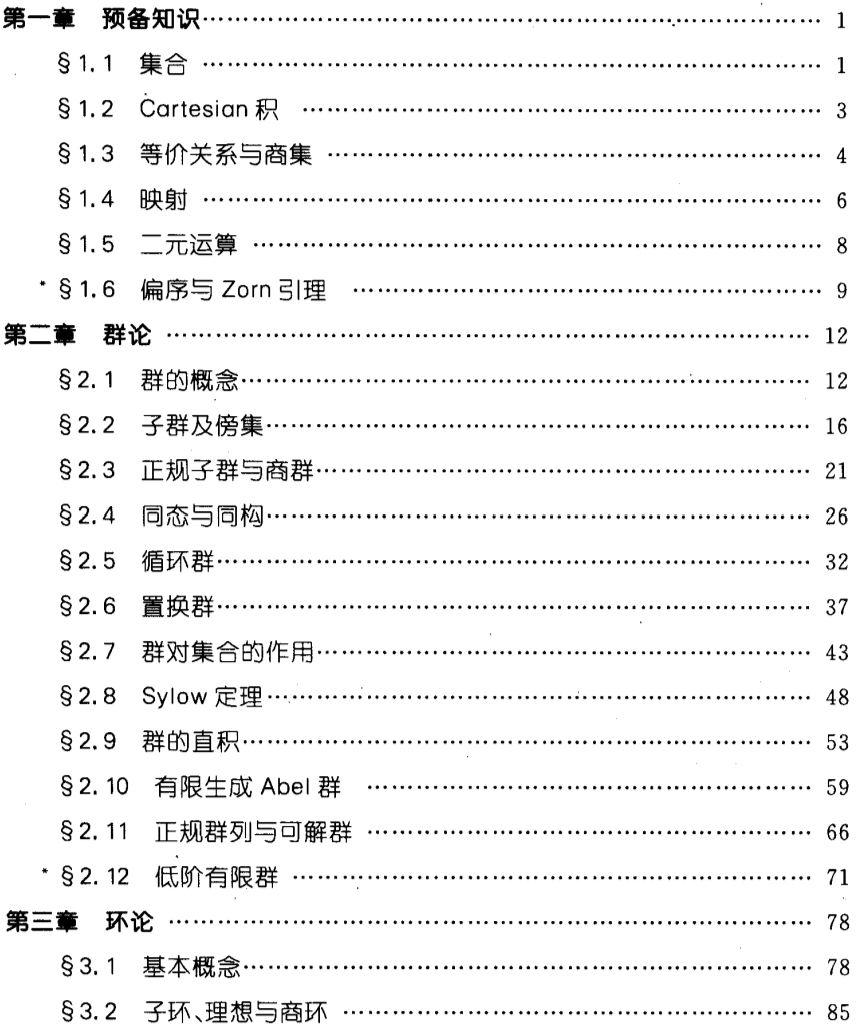
\includegraphics[width=4.6cm]{抽代1.png}
    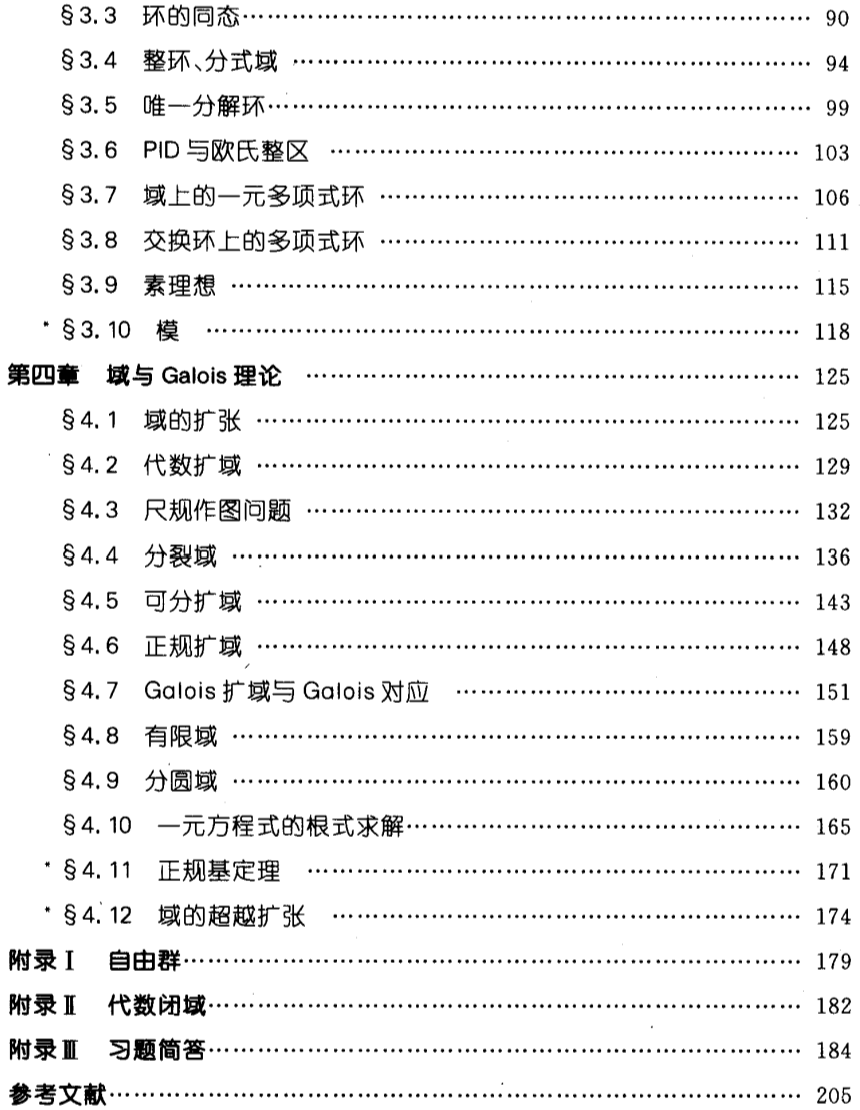
\includegraphics[width=4.6cm]{抽代2.png}
  \end{center}
  各位猜猜我们能讲多少？
\end{frame}

\begin{frame}{三个台阶}
  先回到各位能看懂的语言，数字的世界是怎么一点点变抽象的？
  \begin{block}{我们是怎么一步步走上来的}
    \begin{itemize}
      \item 小学：只用数字。\quad $3 + 5 = 8$
      \item 初中：开始用字母代替数。\quad $a + b = b + a$
      \item 抽象代数：连「运算」本身也用字母代替。
    \end{itemize}
  \end{block}
\end{frame}

\begin{frame}{这门课有两个约定}
  \begin{block}{约定}
    \begin{itemize}
      \item 我们尽量少记忆一些术语和定义；
      \item 只看生活里的例子：钟表、体育课、三角形、正方形、身份证。
    \end{itemize}
  \end{block}

  \begin{att}
    第 12 课，你要自己证明一个三百多年前的定理。
  \end{att}
\end{frame}

% ============================================================================
\section{生活里的两个例子}

\begin{frame}{例子一：体育课上的队形}
  \begin{block}{问题}
    体育课上，老师要把两列纵队变成四列纵队，他做了什么？
  \end{block}

\end{frame}

\begin{frame}{例子二：半夜 12 点}
  \begin{block}{问题}
    为什么半夜 12 点，既叫 0 点，又叫 24 点？
  \end{block}
\begin{center}
  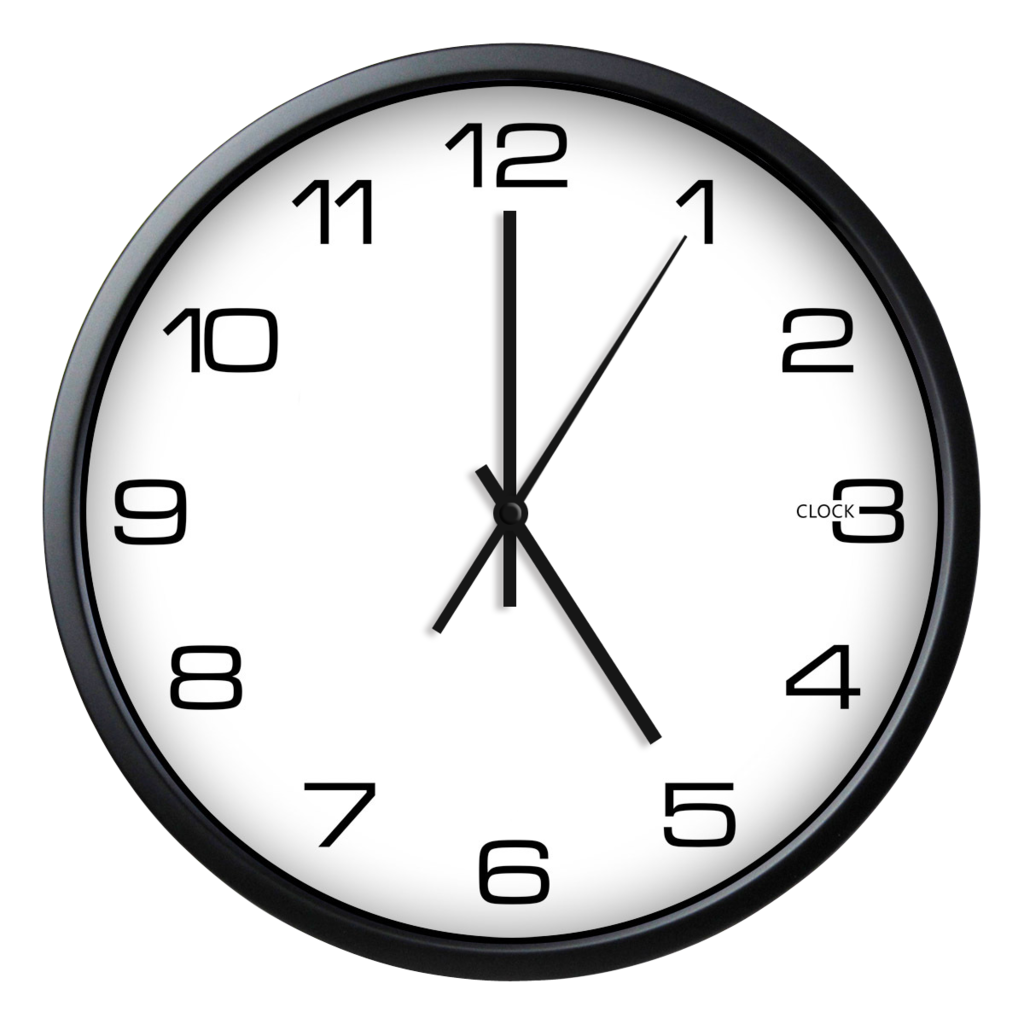
\includegraphics[width=4cm]{时钟.png}
\end{center}

\end{frame}

\begin{frame}{两个例子有什么关系？}
  \begin{itemize}
    \item 队形：人没变，位置上重新排了一遍。
    \item 时间：表没变，指针绕了一圈。
  \end{itemize}

  \begin{block}{共同点}
    东西没变，只是“重新排了一下”。
  \end{block}
    这门课要做的，就是把这句话说清楚。
\end{frame}

% ============================================================================
\section{集合初步}

\begin{frame}{集合是什么}
  \begin{definition}[集合]
    把确定的一堆东西放在一起，就叫做一个集合，用大括号写出来。
  \end{definition}

  \begin{example}
    \(\{1, 2, 3\}\)；\quad \{甲, 乙, 丙\}；\quad \{红, 黄, 蓝\}

    所有的有理数放在一起也是集合；

    自然数、整数也都可以看作集合。
  \end{example}

  \begin{att}
    反过来看一个反例：「我们班个子比较高的同学」不是一个集合。
    因为「比较高」不确定，谁算高、谁不算高，没有统一标准。
    换成「我们班身高超过 160 cm 的同学」就是一个集合了——标准是确定的。
  \end{att}

\end{frame}

\begin{frame}{这节课立刻就能用的写法}
  \begin{itemize}
    \item \(\{1, 2, 3, \dots, 12\}\) —— 钟面上的 12 个时刻
    \item \(\{A, B, C\}\) —— 三角形的三个顶点
    \item \{原地不动, 转 \(90^\circ\), 转 \(180^\circ\), 转 \(270^\circ\)\} —— 正方形的四种转法
  \end{itemize}

  \begin{att}
    注意最后一行：那四个“动作”本身被装进了一个集合里。
  \end{att}
\end{frame}

% ============================================================================
\section{一个悬念}

\begin{frame}{999999 能被 7 整除吗？}

  \begin{block}{问题}
    \[
      999999 \div 7 = ？
    \]
  \end{block}
  \begin{block}{答案}
    \[
      999999 \div 7 = 142857
    \]
    正好整除，一点不剩。
  \end{block}
\end{frame}

\begin{frame}{为什么？}
  \begin{block}{关键线索}
    \[
      999999 = 1000000 - 1 = 10^{6} - 1
    \]
  \end{block}

  \begin{itemize}
    \item 于是问题变成：为什么 \(10^{6} - 1\) 能被 7 整除？
    \item 这件事和 7 有什么关系？把7换成别的会管用吗？
  \end{itemize}


\end{frame}

\begin{frame}{顺便看一个把戏}

  \begin{block}{把 142857 乘上\(k\)看看}

     \begin{columns}[T]  % T=顶部对齐, c=居中, b=底部
       \begin{column}{0.48\textwidth}
          \begin{itemize}
            \item $142857 \times 1 = 142857$
            \item $142857 \times 2 = 285714$
            \item $142857 \times 3 = 428571$
          \end{itemize}
    \end{column}
    \begin{column}{0.48\textwidth}
 \begin{itemize}
      \item $142857 \times 4 = 571428$
      \item $142857 \times 5 = 714285$
      \item $142857 \times 6 = 857142$
    \end{itemize}
    \end{column}
  \end{columns}
  \end{block}
  \pause
    数字还是那六个，只是换了个位置。
\end{frame}

% ============================================================================
\section{这门课要去哪}

\begin{frame}{四站路——课程大纲}
  \begin{itemize}
    \item \textbf{第一站　钟表与取余}：数着数着，会绕回来。
    \item \textbf{第二站　三角形与正方形}：位置换一换，还是那几个样子。
    \item \textbf{第三站　换位置的算术}：先做这个再做那个，结果会不一样。
    \item \textbf{第四站　费马小定理}：回到今天那个 999999。
  \end{itemize}

\end{frame}

\begin{frame}{最后一节课，你会带走三样东西}
  \begin{itemize}
    \item 一个能自己证明的定理（费马小定理）；
    \item 一套看世界的办法：把不同事情里相同的规矩挑出来；
    \item 一个终于能回答的问题：999999 为什么能被 7 整除。
  \end{itemize}

  \vspace{0.6em}
  \begin{center}
    {\large\textcolor{textgreen}{\bfseries 我们从一个最笨的动作开始——数数。}}
  \end{center}
\end{frame}
\begin{frame}{如果你想读一点参考书}
  这些书你大概率是读不懂的，至少也得上了高中：
  \begin{itemize}
    \item 人民教育出版社, 普通高中课程标准实验教科书 数学 选修 3-4 A版 对称与群[M]. 北京: 人民教育出版社, 2007.
    \item 韩士安, 林磊. 近世代数[M]. 2版. 北京: 科学出版社, 2009.
    \item 内森·卡特. 群论: 彩图版[M]. 郭小强, 罗翠玲, 译. 北京: 机械工业出版社, 2019.
    \item LEE G T. Abstract algebra: an introductory course[M]. Cham: Springer, 2018.
  \end{itemize}
  
\end{frame}
% ---------------- 结尾页 ----------------
\begin{frame}
  \begin{center}
    \vspace{1.6cm}
    {\Large\textcolor{textgreen}{\bfseries 下课}}

    \vspace{1.0cm}
    {\large\textcolor{accentgreen}{下节课：从余数到模运算}}
  \end{center}
\end{frame}

\end{document}
